%=======================================================
% CHAPTER 3: CYCLIC CODES
%=======================================================

\begin{frame}[plain]
  \begin{center}\bfseries\centering
    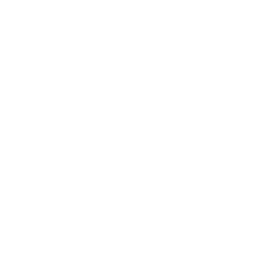
\includegraphics[scale=1]{assets/branding/opa0}
    \vspace{-5.75cm}\\
    {\adjustbox{scale=2.15}{\color{TealDarkCyan}\;IV.\;Cyclic Codes}}
    \bigskip\bigskip
    {\ }\vspace{4cm}\\
    \bigskip
  \end{center}
\end{frame}

%--- NEW: What Does Cyclic Mean? ---
\begin{frame}{\textbf{IV. Cyclic Codes}}{What Does ``Cyclic'' Mean?}
\small
\begin{columns}[T,onlytextwidth]
  \begin{column}{.52\textwidth}
    \textcolor{TealDarkCyan}{\textbf{The core symmetry}}

    A cyclic code is closed under \textbf{rotating} the codeword one position to the right.

    \medskip
    \begin{center}
    \begin{tikzpicture}[scale=0.82]
      % Original codeword
      \foreach \i/\v in {1/1,2/0,3/1,4/1,5/0,6/1,7/0} {
        \pgfmathsetmacro{\xp}{(\i-1)*0.72}
        \node[draw=TealDarkCyan, fill=TealDarkCyan!15, rounded corners=3pt,
              minimum size=0.65cm, font=\small] at (\xp,0.5) {$\v$};
      }
      \node[left=4pt, font=\small, TealDarkCyan] at (-0.1,0.5) {$c=$};
      % Arrow showing rotation
      \draw[-Stealth, AccentCyan, thick] (4.5,0.3) -- (4.5,-0.05)
        node[right=2pt,font=\scriptsize]{rotate};
      % Rotated codeword
      \foreach \i/\v in {1/0,2/1,3/0,4/1,5/1,6/0,7/1} {
        \pgfmathsetmacro{\xp}{(\i-1)*0.72}
        \node[draw=AccentCyan, fill=AccentCyan!15, rounded corners=3pt,
              minimum size=0.65cm, font=\small] at (\xp,-0.5) {$\v$};
      }
      \node[left=4pt, font=\small, AccentCyan] at (-0.1,-0.5) {$c'=$};
    \end{tikzpicture}
    \end{center}

    \medskip
    If $c = (c_0, c_1, \ldots, c_{n-1})$ is a codeword, so is
    \[
      c' = (c_{n-1}, c_0, c_1, \ldots, c_{n-2}).
    \]
    Applying the shift repeatedly generates all cyclic shifts of $c$ — and all must be in the code.
  \end{column}
  \begin{column}{.45\textwidth}
    \textcolor{TealDarkCyan}{\textbf{Why is this useful?}}
    \begin{itemize}
      \item Shift $=$ multiply by $X$ in the polynomial ring
      \item Stability under shifts $=$ ideal in $R_n$
      \item Ideals are generated by a single \emph{generator polynomial} $g(X)$
      \item Encoding $=$ multiply by $g(X)$ — a simple operation
    \end{itemize}

    \bigskip
    \defbox[Hardware bonus]{
    Cyclic codes can be encoded and decoded with \textbf{shift registers} — fast, cheap circuits. This is why they dominate in hardware applications (CRC, CD, satellite).
    }
  \end{column}
\end{columns}
\end{frame}

\begin{frame}{\textbf{IV. Cyclic Codes}}{Cyclic shift}
\small
\defbox[Cyclic code]{
A linear code $\code\le\F_q^n$ is cyclic if
\[
  (c_0,c_1,\ldots,c_{n-1})\in\code
  \quad\Rightarrow\quad
  (c_{n-1},c_0,\ldots,c_{n-2})\in\code.
\]
}
\begin{itemize}
  \item This is invariance under a single permutation.
  \item Since the permutation has order $n$, cyclic codes are modules over a cyclic group algebra.
  \item The polynomial model makes this precise.
\end{itemize}
\end{frame}

\begin{frame}{\textbf{IV. Cyclic Codes}}{Polynomial dictionary}
\small
\defbox[Vector to polynomial]{
Identify
\[
  (c_0,c_1,\ldots,c_{n-1})
  \quad\longleftrightarrow\quad
  c(X)=c_0+c_1X+\cdots+c_{n-1}X^{n-1}.
\]
}
\begin{itemize}
  \item Multiplication by $X$ shifts coefficients.
  \item The relation $X^n=1$ performs wrap-around.
  \item Therefore we work modulo $X^n-1$.
\end{itemize}
\end{frame}

\begin{frame}{\textbf{IV. Cyclic Codes}}{The quotient ring}
\small
\defbox[Ambient ring]{
\[
  R_n=\F_q[X]/(X^n-1).
\]
}
\begin{itemize}
  \item Vectors of length $n$ are polynomials of degree $<n$.
  \item Cyclic shift is multiplication by $X$ in $R_n$.
  \item A cyclic code is an $\F_q$-subspace stable under multiplication by $X$.
\end{itemize}
\begin{block}{Key question}
Which subspaces of $R_n$ are stable under multiplication by $X$?
\end{block}
\end{frame}

%--- NEW: R_n as a Rotation Carousel ---
\begin{frame}{\textbf{IV. Cyclic Codes}}{$R_n$: The Ring as a Rotation}
\small
\begin{columns}[T,onlytextwidth]
  \begin{column}{.46\textwidth}
    Think of $R_n = \F_q[X]/(X^n-1)$ like a \textbf{clock with $n$ positions} $0,1,\ldots,n-1$.

    \medskip
    Multiplying by $X$ = \textbf{rotating one step}.

    \medskip
    \begin{center}
    \begin{tikzpicture}[scale=1.0]
      % Draw a heptagon (n=7 clock)
      \def\R{1.45}
      \foreach \i in {0,...,6} {
        \pgfmathsetmacro{\ang}{90 - \i*360/7}
        \pgfmathsetmacro{\px}{\R*cos(\ang)}
        \pgfmathsetmacro{\py}{\R*sin(\ang)}
        \fill[TealDarkCyan] (\px,\py) circle (2.8pt);
        \node[font=\tiny\bfseries, TealDarkCyan,
              xshift={0.28cm*cos(\ang)}, yshift={0.28cm*sin(\ang)}]
          at (\px,\py) {$X^{\i}$};
      }
      % Draw the clock circle
      \draw[TealDarkCyan!40, thick] (0,0) circle (\R);
      % Rotation arrow (curved, at top)
      \draw[-Stealth, AccentCyan, thick, bend left=30]
        ({(\R+0.12)*cos(90)},{(\R+0.12)*sin(90)})
        to node[above=2pt,font=\tiny]{$\times X$}
        ({(\R+0.12)*cos(90-360/7)},{(\R+0.12)*sin(90-360/7)});
      % X^7=1 label
      \node[font=\scriptsize, TealDarkCyan] at (0,-0.1) {$X^7=1$};
    \end{tikzpicture}
    \end{center}
  \end{column}
  \begin{column}{.51\textwidth}
    \textcolor{TealDarkCyan}{\textbf{From integers to polynomials}}

    \begin{center}
    \begin{tabular}{c|c}
      $\Z/n\Z$ & $\F_q[X]/(X^n{-}1)$ \\\hline
      \rowcolor{TealDarkCyan!8}
      add $n$ to get $0$ & $X^n = 1$ \\
      $+1$ = shift right & $\times X$ = shift \\
      \rowcolor{TealDarkCyan!8}
      subgroup = ideal & subspace closed\\
                       & under $\times X$ = ideal\\
    \end{tabular}
    \end{center}

    \medskip
    \defbox[Why this matters]{
    A cyclic code is a subspace of $R_n$ that is \emph{closed under rotation}. That is exactly an \textbf{ideal} — generated by a single divisor $g(X)$ of $X^n-1$.
    }
  \end{column}
\end{columns}
\end{frame}

\begin{frame}{\textbf{IV. Cyclic Codes}}{Ideals}
\small
\thmbox[Cyclic codes are ideals]{
Under the identification $\F_q^n\cong R_n$, cyclic codes are exactly the ideals of $R_n$.
}
\begin{proof}
If $\code$ is stable under multiplication by $X$, then it is stable under multiplication by every polynomial in $X$. Hence it is an ideal. The converse is immediate.
\end{proof}
\begin{block}{Consequence}
The classification of cyclic codes is an ideal-theoretic problem.
\end{block}
\end{frame}

\begin{frame}{\textbf{IV. Cyclic Codes}}{Principal ideals}
\small
\thmbox[Principal generator]{
Every ideal of $R_n$ is generated by a unique monic divisor $g(X)$ of $X^n-1$:
\[
  \code=(g(X)).
\]
}
\begin{itemize}
  \item This follows from the principal ideal property of $\F_q[X]$.
  \item The generator polynomial is the monic element of least degree in the code.
  \item The divisibility condition is $g(X)\mid X^n-1$.
\end{itemize}
\end{frame}

\begin{frame}{\textbf{IV. Cyclic Codes}}{Dimension}
\small
\thmbox[Dimension formula]{
If $\code=(g(X))\subseteq R_n$ and $\deg g=r$, then
\[
  \dim_{\F_q}\code=n-r.
\]
}
\begin{proof}
The polynomials
\[
  g(X),Xg(X),\ldots,X^{n-r-1}g(X)
\]
form an $\F_q$-basis of the ideal.
\end{proof}
\end{frame}

\begin{frame}{\textbf{IV. Cyclic Codes}}{Generator matrix from shifts}
\small
If
\[
  g(X)=g_0+g_1X+\cdots+g_rX^r,
\]
then a generator matrix is obtained by shifting the coefficient vector:
\[
\begin{bmatrix}
g_0&g_1&\cdots&g_r&0&\cdots&0\\
0&g_0&g_1&\cdots&g_r&\cdots&0\\
\vdots&&\ddots&&&\ddots&\vdots
\end{bmatrix}.
\]
\begin{itemize}
  \item This matrix is Toeplitz-like.
  \item It encodes multiplication by $g(X)$.
\end{itemize}
\end{frame}

%--- NEW: Circulant / Shifted Structure ---
\begin{frame}{\textbf{IV. Cyclic Codes}}{The Shifted (Toeplitz) Structure of the Generator Matrix}
\small
For $g(X)=X^3+X+1$ and the $[7,4,3]$ cyclic code, the generator matrix is:
\[
G = \begin{bmatrix}
\mathbf{1}&\mathbf{1}&\mathbf{0}&\mathbf{1}&0&0&0\\
0&\mathbf{1}&\mathbf{1}&\mathbf{0}&\mathbf{1}&0&0\\
0&0&\mathbf{1}&\mathbf{1}&\mathbf{0}&\mathbf{1}&0\\
0&0&0&\mathbf{1}&\mathbf{1}&\mathbf{0}&\mathbf{1}
\end{bmatrix}
\]

\begin{center}
\begin{tikzpicture}[scale=0.82]
  % Draw the 4x7 matrix as colored cells
  % Row i, col j (0-indexed). Entry is 1 if the row is a shift of [1,1,0,1,0,0,0]
  % Row 0: [1,1,0,1,0,0,0]
  % Row 1: [0,1,1,0,1,0,0]
  % Row 2: [0,0,1,1,0,1,0]
  % Row 3: [0,0,0,1,1,0,1]
  % Entries that are 1 (from g coefficients):
  % Row 0: cols 0,1,3
  % Row 1: cols 1,2,4
  % Row 2: cols 2,3,5
  % Row 3: cols 3,4,6
  \foreach \row in {0,1,2,3} {
    \foreach \col in {0,...,6} {
      \pgfmathsetmacro{\xp}{0.72*\col}
      \pgfmathsetmacro{\yp}{-0.55*\row}
      % check if this cell is 1 or 0
      % Row r has 1s at cols r, r+1, r+3 (mod 7, but since all <7, no mod needed)
      % col == row, row+1, or row+3 → cell is 1; else 0
      % (\d is LaTeX's dot-below accent, so use \da/\db/\dc as safe names)
      \pgfmathtruncatemacro{\da}{\col-\row}
      \pgfmathtruncatemacro{\db}{\col-\row-1}
      \pgfmathtruncatemacro{\dc}{\col-\row-3}
      \ifnum\da=0
        \node[draw=AccentCyan,fill=AccentCyan!22,rounded corners=2pt,
              minimum size=0.62cm,font=\small\bfseries] at (\xp,\yp) {1};
      \else\ifnum\db=0
        \node[draw=AccentCyan,fill=AccentCyan!22,rounded corners=2pt,
              minimum size=0.62cm,font=\small\bfseries] at (\xp,\yp) {1};
      \else\ifnum\dc=0
        \node[draw=AccentCyan,fill=AccentCyan!22,rounded corners=2pt,
              minimum size=0.62cm,font=\small\bfseries] at (\xp,\yp) {1};
      \else
        \node[draw=TealDarkCyan!30,fill=TealDarkCyan!5,rounded corners=2pt,
              minimum size=0.62cm,font=\small] at (\xp,\yp) {0};
      \fi\fi\fi
    }
  }
  % Diagonal shift arrows
  \draw[-Stealth,AccentCyan,dashed,thick]
    (-0.5,-0.0) -- (-0.5,-0.55)
    node[left,font=\tiny]{shift};
\end{tikzpicture}
\end{center}

\vspace{-4pt}
\begin{itemize}
  \item Each row is a \textbf{one-position cyclic shift} of the row above
  \item The non-zero diagonals follow the pattern of $g$'s coefficients $(1,1,0,1)$
  \item This ``staircase'' pattern is what makes encoding a shift-register operation
\end{itemize}
\end{frame}

\begin{frame}{\textbf{IV. Cyclic Codes}}{Parity-check polynomial}
\small
\defbox[Check polynomial]{
If $g(X)\mid X^n-1$, define
\[
  h(X)=\frac{X^n-1}{g(X)}.
\]
}
\begin{itemize}
  \item $\deg h=k$ when $\code$ has dimension $k$.
  \item Since $g(X)h(X)=0$ in $R_n$, multiplication by $h(X)$ checks membership.
  \item More precisely, $c(X)\in(g)$ implies $c(X)h(X)\equiv0\pmod{X^n-1}$.
\end{itemize}
\end{frame}

\begin{frame}{\textbf{IV. Cyclic Codes}}{Reciprocal polynomials}
\small
\defbox[Reciprocal]{
For $f(X)=f_0+\cdots+f_mX^m$ with $f_0\ne0$, define
\[
  f^*(X)=X^mf(X^{-1}).
\]
}
\begin{itemize}
  \item Parity-check matrices are naturally written using reciprocal polynomials.
  \item The dual of a cyclic code is cyclic.
  \item If $\code=(g)$ and $h=(X^n-1)/g$, then $\code^\perp$ is generated by a reciprocal of $h$.
\end{itemize}
\end{frame}

\begin{frame}{\textbf{IV. Cyclic Codes}}{Idempotents}
\small
\defbox[Idempotent generator]{
When $\gcd(n,q)=1$, each cyclic code has a unique idempotent generator $e(X)$ satisfying
\[
  e(X)^2=e(X),\qquad \code=(e(X)).
\]
}
\begin{itemize}
  \item Idempotents decompose the semisimple ring $R_n$.
  \item They expose the representation-theoretic structure.
  \item Generator polynomials are usually better for computation.
\end{itemize}
\end{frame}

\begin{frame}{\textbf{IV. Cyclic Codes}}{Roots}
\small
Let $\alpha$ be an $n$-th root of unity in an extension field.
\begin{itemize}
  \item A cyclic code generated by $g(X)$ has zeros $\alpha^i$ where $g(\alpha^i)=0$.
  \item The defining set is
  \[
    Z(\code)=\{i\pmod n:g(\alpha^i)=0\}.
  \]
  \item Root sets translate algebraic divisibility into combinatorics modulo $n$.
\end{itemize}
\end{frame}

\begin{frame}{\textbf{IV. Cyclic Codes}}{Cyclotomic cosets}
\small
\defbox[Q-cyclotomic coset]{
Modulo $n$, the $q$-cyclotomic coset of $i$ is
\[
  C_i=\{i,iq,iq^2,\ldots\}\pmod n.
\]
}
\begin{itemize}
  \item If $\alpha^i$ is a root over $\F_q$, all conjugates $\alpha^{iq^j}$ are roots.
  \item Therefore defining sets are unions of cyclotomic cosets.
  \item Minimal polynomials correspond to these cosets.
\end{itemize}
\end{frame}

%--- NEW: Cyclotomic Cosets Visual for n=7 ---
\begin{frame}{\textbf{IV. Cyclic Codes}}{Cyclotomic Cosets for $n=7$, $q=2$: Orbits Under $\times 2$}
\small
\begin{columns}[T,onlytextwidth]
  \begin{column}{.50\textwidth}
    Multiplying by $q=2$ modulo $n=7$ partitions $\{0,1,\ldots,6\}$ into orbits:

    \medskip
    \begin{center}
    \begin{tikzpicture}[scale=1.0]
      \def\R{1.5}
      % Draw circle
      \draw[TealDarkCyan!30,thick] (0,0) circle (\R);
      % Place 7 points at positions 0..6
      % Position i at angle 90 - i*360/7
      % C_0 = {0}: gray
      \pgfmathsetmacro{\ang}{90}
      \fill[gray!50] ({\R*cos(\ang)},{\R*sin(\ang)}) circle (4pt);
      \node[font=\scriptsize,gray,xshift={0.32cm*cos(\ang)},yshift={0.32cm*sin(\ang)}]
        at ({\R*cos(\ang)},{\R*sin(\ang)}) {$0$};
      % C_1 = {1,2,4}: TealDarkCyan
      \foreach \i in {1,2,4} {
        \pgfmathsetmacro{\ang}{90-\i*360/7}
        \fill[TealDarkCyan] ({\R*cos(\ang)},{\R*sin(\ang)}) circle (4pt);
        \node[font=\scriptsize\bfseries,TealDarkCyan,
              xshift={0.32cm*cos(\ang)},yshift={0.32cm*sin(\ang)}]
          at ({\R*cos(\ang)},{\R*sin(\ang)}) {$\i$};
      }
      % C_3 = {3,5,6}: AccentCyan
      \foreach \i in {3,5,6} {
        \pgfmathsetmacro{\ang}{90-\i*360/7}
        \fill[AccentCyan] ({\R*cos(\ang)},{\R*sin(\ang)}) circle (4pt);
        \node[font=\scriptsize\bfseries,AccentCyan,
              xshift={0.32cm*cos(\ang)},yshift={0.32cm*sin(\ang)}]
          at ({\R*cos(\ang)},{\R*sin(\ang)}) {$\i$};
      }
      % Orbit arrows for C_1: 1->2->4->1
      \pgfmathsetmacro{\aone}{90-1*360/7}
      \pgfmathsetmacro{\atwo}{90-2*360/7}
      \pgfmathsetmacro{\afour}{90-4*360/7}
      \draw[-Stealth,TealDarkCyan,thick,bend left=15]
        ({\R*cos(\aone)},{\R*sin(\aone)}) to ({\R*cos(\atwo)},{\R*sin(\atwo)});
      \draw[-Stealth,TealDarkCyan,thick,bend left=15]
        ({\R*cos(\atwo)},{\R*sin(\atwo)}) to ({\R*cos(\afour)},{\R*sin(\afour)});
      \draw[-Stealth,TealDarkCyan,thick,bend left=15]
        ({\R*cos(\afour)},{\R*sin(\afour)}) to ({\R*cos(\aone)},{\R*sin(\aone)});
      % Orbit arrows for C_3: 3->6->5->3
      \pgfmathsetmacro{\athree}{90-3*360/7}
      \pgfmathsetmacro{\asix}{90-6*360/7}
      \pgfmathsetmacro{\afive}{90-5*360/7}
      \draw[-Stealth,AccentCyan,thick,bend right=15]
        ({\R*cos(\athree)},{\R*sin(\athree)}) to ({\R*cos(\asix)},{\R*sin(\asix)});
      \draw[-Stealth,AccentCyan,thick,bend right=15]
        ({\R*cos(\asix)},{\R*sin(\asix)}) to ({\R*cos(\afive)},{\R*sin(\afive)});
      \draw[-Stealth,AccentCyan,thick,bend right=15]
        ({\R*cos(\afive)},{\R*sin(\afive)}) to ({\R*cos(\athree)},{\R*sin(\athree)});
      % Label ×2
      \node[font=\tiny,TealDarkCyan] at (0.55,0.35) {$\times2$};
      \node[font=\tiny,AccentCyan]   at (-0.55,-0.35) {$\times2$};
    \end{tikzpicture}
    \end{center}
  \end{column}
  \begin{column}{.47\textwidth}
    \textcolor{TealDarkCyan}{\textbf{Three cosets:}}

    \begin{tabular}{c|c|l}
      Coset & Elements & Min. poly \\\hline
      \rowcolor{TealDarkCyan!8}
      $C_0$ & $\{0\}$ & $X+1$ \\
      $C_1$ & $\{1,2,4\}$ & $X^3+X+1$ \\
      \rowcolor{TealDarkCyan!8}
      $C_3$ & $\{3,5,6\}$ & $X^3+X^2+1$ \\
    \end{tabular}

    \medskip
    This gives the factorization:
    \[
      X^7-1 = \underbrace{(X+1)}_{C_0}\underbrace{(X^3+X+1)}_{C_1}\underbrace{(X^3+X^2+1)}_{C_3}
    \]

    \smallskip
    \textbf{Cyclic codes} = choose a subset of factors as the generator $g(X)$.
  \end{column}
\end{columns}
\end{frame}

\begin{frame}{\textbf{IV. Cyclic Codes}}{Minimal polynomials}
\small
\defbox[Minimal polynomial]{
For $\alpha^i$, the minimal polynomial over $\F_q$ is
\[
  M_i(X)=\prod_{j\in C_i}(X-\alpha^j).
\]
}
\begin{itemize}
  \item It lies in $\F_q[X]$.
  \item It is irreducible.
  \item Generator polynomials of cyclic codes are products of such $M_i(X)$.
\end{itemize}
\end{frame}

\begin{frame}{\textbf{IV. Cyclic Codes}}{BCH codes}
\small
\defbox[BCH design]{
A BCH code is a cyclic code whose generator polynomial has a prescribed block of consecutive roots.
}
\[
  g(\alpha^b)=g(\alpha^{b+1})=\cdots=g(\alpha^{b+\delta-2})=0.
\]
\begin{itemize}
  \item The integer $\delta$ is the designed distance.
  \item Consecutive roots force many syndromes to vanish.
  \item The BCH bound converts this into a distance guarantee.
\end{itemize}
\end{frame}

%--- NEW: BCH Roots on the Circle ---
\begin{frame}{\textbf{IV. Cyclic Codes}}{BCH Design: Consecutive Roots on the Circle}
\small
\begin{columns}[T,onlytextwidth]
  \begin{column}{.48\textwidth}
    \textbf{Idea:} place $n$ roots of unity on a circle. Prescribe $\delta-1$ \textcolor{AccentCyan}{\textbf{consecutive}} ones as roots of $g(X)$. The BCH bound guarantees $d \ge \delta$.

    \medskip
    \begin{center}
    \begin{tikzpicture}[scale=0.85]
      % Unit circle
      \draw[TealDarkCyan!30,thick] (0,0) circle (1.5);
      % n=7 roots, labeled alpha^0..alpha^6
      \foreach \i in {0,...,6} {
        \pgfmathsetmacro{\ang}{90-\i*360/7}
        \pgfmathsetmacro{\px}{1.5*cos(\ang)}
        \pgfmathsetmacro{\py}{1.5*sin(\ang)}
        \ifnum\i=0
          \fill[gray] (\px,\py) circle (3.2pt);
          \node[font=\tiny,gray,xshift={0.3cm*cos(\ang)},yshift={0.3cm*sin(\ang)}]
            at (\px,\py) {$\alpha^0$};
        \else\ifnum\i=1
          \fill[AccentCyan] (\px,\py) circle (4pt);
          \node[font=\tiny\bfseries,AccentCyan,xshift={0.3cm*cos(\ang)},yshift={0.3cm*sin(\ang)}]
            at (\px,\py) {$\alpha^1$};
        \else\ifnum\i=2
          \fill[AccentCyan] (\px,\py) circle (4pt);
          \node[font=\tiny\bfseries,AccentCyan,xshift={0.3cm*cos(\ang)},yshift={0.3cm*sin(\ang)}]
            at (\px,\py) {$\alpha^2$};
        \else
          \fill[TealDarkCyan!50] (\px,\py) circle (3pt);
          \node[font=\tiny,TealDarkCyan!70,xshift={0.3cm*cos(\ang)},yshift={0.3cm*sin(\ang)}]
            at (\px,\py) {$\alpha^{\i}$};
        \fi\fi\fi
      }
      % Arc highlighting the 2 consecutive roots (delta-1=2)
      \draw[AccentCyan,very thick]
        ({1.65*cos(90-1*360/7)},{1.65*sin(90-1*360/7)})
        arc[radius=1.65, start angle={90-1*360/7}, end angle={90-2*360/7}];
      \node[font=\tiny,AccentCyan] at (1.3,0.8) {$\delta{-}1=2$};
    \end{tikzpicture}
    \end{center}
  \end{column}
  \begin{column}{.49\textwidth}
    \textcolor{TealDarkCyan}{\textbf{BCH codes with $n=7$, $q=2$:}}

    \medskip
    \begin{tabular}{c|l|c|c}
      $\delta$ & roots of $g$ & $[n,k]$ & $d$ \\\hline
      \rowcolor{TealDarkCyan!8}
      3 & $\alpha^1,\alpha^2$ & $[7,4]$ & 3 (Hamming) \\
      5 & $\alpha^1,\ldots,\alpha^4$ & $[7,1]$ & 7 (repetition) \\
    \end{tabular}

    \medskip
    \begin{block}{BCH Bound}
    $\delta-1$ consecutive roots $\Rightarrow d \ge \delta$. More prescribed roots $\Rightarrow$ higher designed distance $\Rightarrow$ lower rate.
    \end{block}

    \medskip
    \textcolor{TealDarkCyan}{\textbf{Key insight for non-majors:}} prescribing more roots forces the codeword polynomial to have more zeros, which ``spreads'' the code and increases the minimum distance — at the cost of fewer codewords (lower rate).
  \end{column}
\end{columns}
\end{frame}

\begin{frame}{\textbf{IV. Cyclic Codes}}{BCH bound}
\small
\thmbox[BCH bound]{
If a cyclic code has $\delta-1$ consecutive roots
\[
  \alpha^b,\alpha^{b+1},\ldots,\alpha^{b+\delta-2},
\]
then its minimum distance is at least $\delta$.
}
\begin{proof}
A codeword of weight $<\delta$ would give a nonzero polynomial with too many consecutive zero syndromes, forcing a Vandermonde determinant to vanish.
\end{proof}
\end{frame}

\begin{frame}{\textbf{IV. Cyclic Codes}}{Narrow-sense primitive BCH}
\small
\defbox[Common special case]{
Let $n=q^m-1$ and let $\alpha$ be primitive in $\F_{q^m}$. The narrow-sense BCH code of designed distance $\delta$ has roots
\[
  \alpha,\alpha^2,\ldots,\alpha^{\delta-1}.
\]
}
\begin{itemize}
  \item Primitive: the length is the full multiplicative order.
  \item Narrow-sense: the first root is $\alpha$.
  \item Hamming codes occur when $\delta=3$ in the binary case.
\end{itemize}
\end{frame}

\begin{frame}{\textbf{IV. Cyclic Codes}}{Cyclic Hamming code}
\small
Let $n=2^r-1$ and let $\alpha\in\F_{2^r}$ be primitive.
\begin{itemize}
  \item Let $g(X)$ be the minimal polynomial of $\alpha$ over $\F_2$.
  \item Then $\deg g=r$.
  \item The cyclic code $(g)$ has parameters
  \[
    [2^r-1,2^r-1-r,3]_2.
  \]
\end{itemize}
\begin{block}{Identification}
This is the binary Hamming code in cyclic coordinates.
\end{block}
\end{frame}

\begin{frame}{\textbf{IV. Cyclic Codes}}{The case n equals 7}
\small
Over $\F_2$,
\[
  X^7-1=(X+1)(X^3+X+1)(X^3+X^2+1).
\]
\begin{itemize}
  \item A primitive $7$-th root has minimal polynomial $X^3+X+1$ or $X^3+X^2+1$.
  \item Either cubic gives a cyclic $[7,4,3]$ Hamming code.
  \item The two choices are equivalent under coordinate reversal.
\end{itemize}
\end{frame}

\begin{frame}{\textbf{IV. Cyclic Codes}}{Encoding by multiplication}
\small
For a cyclic code $(g)$ with $\deg g=r$, non-systematic encoding is
\[
  m(X)\longmapsto c(X)=m(X)g(X),\qquad \deg m< n-r.
\]
\begin{itemize}
  \item The message polynomial has $k=n-r$ coefficients.
  \item The product automatically lies in the ideal $(g)$.
  \item Hardware can implement this multiplication by shift registers.
\end{itemize}
\end{frame}

\begin{frame}{\textbf{IV. Cyclic Codes}}{Systematic cyclic encoding}
\small
Let $\deg g=r$. To encode a message $m(X)$ with $\deg m<k$:
\[
  X^r m(X)=q(X)g(X)+p(X),\qquad \deg p<r.
\]
Then set
\[
  c(X)=X^rm(X)-p(X).
\]
\begin{itemize}
  \item Since $c(X)$ is divisible by $g(X)$, it is a codeword.
  \item The high-degree coefficients contain the message.
  \item The low-degree polynomial $p(X)$ supplies parity.
\end{itemize}
\end{frame}

%--- NEW: Systematic Encoding Walkthrough ---
\begin{frame}{\textbf{IV. Cyclic Codes}}{Systematic Encoding: Step-by-Step Example}
\small
Encode message $m(X) = X^3 + 1$ (i.e.\ $m=(1,0,0,1)$) using $g(X)=X^3+X+1$.

\medskip
\begin{center}
\begin{tikzpicture}[scale=0.88,
  sbox/.style={draw=TealDarkCyan,thick,rounded corners=4pt,
               fill=TealDarkCyan!8,minimum width=5.2cm,
               minimum height=0.55cm,font=\scriptsize,align=left}]
  \node[sbox] at (0,3.4) {\textbf{Step 1.} Form $X^3 m(X) = X^6+X^3$};
  \node[sbox] at (0,2.75) {\textbf{Step 2.} Divide: $X^6+X^3 = (X^3+X^2+X+1)\cdot g(X) + (X^2+X)$};
  \node[sbox,fill=AccentCyan!10,draw=AccentCyan] at (0,2.1)
    {\textbf{Step 3.} Remainder $p(X) = X^2+X$ (the parity part)};
  \node[sbox] at (0,1.45)
    {\textbf{Step 4.} Codeword: $c(X)=X^3 m(X)-p(X)=X^6+X^3+X^2+X$};
  \node[sbox,fill=TealDarkCyan!15] at (0,0.8)
    {\textbf{Check:} $c(X)\div g(X)=(X^3+X^2+X+1)$ — remainder 0 \checkmark};
\end{tikzpicture}
\end{center}

\vspace{-2pt}
\begin{columns}[T,onlytextwidth]
  \begin{column}{.50\textwidth}
    \textbf{Codeword in vector form:}
    \[
      c = (0,1,1,1,0,0,1) \in \F_2^7
    \]
    \begin{itemize}
      \item Bits 4--7 (positions $X^3,\ldots,X^6$): the message $(1,0,0,1)$
      \item Bits 1--3: the parity $(0,1,1)$ from $p(X)=X^2+X$
    \end{itemize}
  \end{column}
  \begin{column}{.47\textwidth}
    \begin{block}{Why this works}
    Since $c(X) = X^3 m(X) - p(X)$ and $p(X) \equiv X^3 m(X) \pmod{g}$, we get $c(X) \equiv 0 \pmod{g}$. So $c$ is a codeword.
    \end{block}
  \end{column}
\end{columns}
\end{frame}

\begin{frame}{\textbf{IV. Cyclic Codes}}{Syndrome polynomial}
\small
For received $v(X)=c(X)+e(X)$, compute the remainder
\[
  s(X)=v(X)\bmod g(X).
\]
\begin{itemize}
  \item Since $c(X)$ is divisible by $g(X)$, $s(X)=e(X)\bmod g(X)$.
  \item This is the polynomial analogue of $Hv^T=He^T$.
  \item BCH decoding refines this by evaluating at roots of $g$.
\end{itemize}
\end{frame}

\begin{frame}{\textbf{IV. Cyclic Codes}}{Root syndromes}
\small
If $\alpha^i$ is a root of $g(X)$, then every codeword satisfies
\[
  c(\alpha^i)=0.
\]
For $v=c+e$,
\[
  v(\alpha^i)=e(\alpha^i).
\]
\begin{itemize}
  \item The numbers $S_i=v(\alpha^i)$ are syndromes.
  \item Decoding asks for the error locations and values from these sums.
  \item This is a finite-field moment problem.
\end{itemize}
\end{frame}

\begin{frame}{\textbf{IV. Cyclic Codes}}{Error locator polynomial}
\small
For error locations $j_1,\ldots,j_t$, define
\[
  \Lambda(Z)=\prod_{\ell=1}^t(1-\alpha^{j_\ell}Z).
\]
\begin{itemize}
  \item The roots of $\Lambda$ identify error locations.
  \item BCH and Reed--Solomon decoding compute $\Lambda$ from syndromes.
  \item Berlekamp--Massey is an efficient algorithm for this recurrence problem.
\end{itemize}
\end{frame}

\begin{frame}{\textbf{IV. Cyclic Codes}}{LFSR viewpoint}
\small
\defbox[Linear feedback shift register]{
Division by $g(X)$ can be implemented with a shift register whose feedback taps are the nonzero coefficients of $g(X)$.
}
\begin{itemize}
  \item Memory cost is $\deg g=n-k$ registers.
  \item Input is processed one symbol per clock.
  \item This is why cyclic codes became central in hardware error control.
\end{itemize}
\end{frame}

%--- NEW: LFSR Circuit Diagram ---
\begin{frame}{\textbf{IV. Cyclic Codes}}{The LFSR Circuit for $g(X)=X^3+X+1$}
\small
For the $[7,4,3]$ cyclic Hamming code, $g(X)=X^3+X+1$. The feedback taps are at $X^0$ and $X^1$.

\medskip
\begin{center}
\begin{tikzpicture}[
  reg/.style  = {draw=TealDarkCyan, thick, rectangle,
                 minimum width=0.9cm, minimum height=0.7cm, fill=TealDarkCyan!12},
  xorcirc/.style = {draw=AccentCyan, thick, circle,
                    minimum size=0.5cm, fill=AccentCyan!15, font=\small},
  arr/.style  = {-Stealth, thick, TealDarkCyan},
  farr/.style = {-Stealth, thick, AccentCyan, dashed}
]
  % Input node
  \node[font=\small] (inp) at (-2.5,0) {input $b_i$};
  % XOR gates
  \node[xorcirc] (x1) at (-1.2,0) {$\oplus$};
  \node[xorcirc] (x2) at ( 1.4,0) {$\oplus$};
  % Registers R0, R1, R2
  \node[reg] (R0) at (0,   0) {$R_0$};
  \node[reg] (R1) at (2.6, 0) {$R_1$};
  \node[reg] (R2) at (4.6, 0) {$R_2$};
  % Forward connections
  \draw[arr] (inp) -- (x1);
  \draw[arr] (x1)  -- (R0);
  \draw[arr] (R0)  -- (x2);
  \draw[arr] (x2)  -- (R1);
  \draw[arr] (R1)  -- (R2);
  \node[right=4pt,font=\small] at (R2.east) {$\to$ parity out};
  % Feedback from R2 back to x1 (tap for $g_0=1$, i.e.\ $X^0$)
  \draw[farr] (R2.south) -- ++(0,-0.55) -| (x1.south)
    node[near start, below, font=\tiny, AccentCyan]{tap $X^0$};
  % Feedback from R2 back to x2 (tap for $g_1=1$, i.e.\ $X^1$)
  \draw[farr] (R2.south)++(0,-0.55) -- ++(0,0) -| (x2.south)
    node[near end, below, font=\tiny, AccentCyan]{tap $X^1$};
  % Label
  \node[font=\scriptsize, TealDarkCyan] at (1.15,-1.4)
    {Computes remainder of $X^3 \cdot m(X) \div g(X)$ — one bit per clock};
\end{tikzpicture}
\end{center}

\begin{columns}[T,onlytextwidth]
  \begin{column}{.48\textwidth}
    \textbf{Encoding (4 clock cycles):}
    \begin{enumerate}\small
      \item Feed in the $4$ message bits $m_3,m_2,m_1,m_0$
      \item The 3 registers accumulate the parity
      \item Read off $(R_0, R_1, R_2)$ — these are the 3 parity bits
    \end{enumerate}
  \end{column}
  \begin{column}{.48\textwidth}
    \textbf{Key advantage:}
    \begin{itemize}\small
      \item Only $r = n{-}k$ flip-flops needed
      \item One XOR gate per feedback tap
      \item Works at wire speed — no computation delay
      \item Used in every USB, Ethernet, and SATA controller
    \end{itemize}
  \end{column}
\end{columns}
\end{frame}

\begin{frame}{\textbf{IV. Cyclic Codes}}{Burst errors}
\small
\defbox[Burst]{
A burst of length $\ell$ is an error whose nonzero positions lie in $\ell$ consecutive coordinates.
}
\begin{itemize}
  \item Polynomial remainders are well suited for burst detection.
  \item CRC polynomials are chosen to detect common burst patterns.
  \item This is detection rather than correction in many communication protocols.
\end{itemize}
\end{frame}

\begin{frame}{\textbf{IV. Cyclic Codes}}{CRC codes}
\small
CRC uses a generator polynomial $g(X)$ and transmits a multiple of $g(X)$.
\begin{itemize}
  \item Receiver divides by $g(X)$.
  \item Nonzero remainder means an error was detected.
  \item The method is a cyclic-code membership test.
\end{itemize}
\begin{block}{Mathematical core}
CRC is not a different theory: it is cyclic codes used primarily for error detection.
\end{block}
\end{frame}

%--- NEW: CRC in Daily Life ---
\begin{frame}{\textbf{IV. Cyclic Codes}}{CRC in Your Daily Life}
\small
\begin{columns}[T,onlytextwidth]
  \begin{column}{.52\textwidth}
    \textcolor{TealDarkCyan}{\textbf{Every data transfer uses CRC.}}

    \medskip
    \begin{tabular}{p{2.3cm}|p{1.4cm}|p{1.5cm}}
      \textbf{Standard} & \textbf{Polynomial} & \textbf{Detects} \\\hline
      \rowcolor{TealDarkCyan!8}
      Ethernet (CRC-32) & $x^{32}+\cdots$ & $\le 32$-bit bursts \\
      USB 2.0 & CRC-16 & $\le 16$-bit bursts \\
      \rowcolor{TealDarkCyan!8}
      SATA/NVMe & CRC-32 & storage errors \\
      PNG / ZIP & CRC-32 & file corruption \\
      \rowcolor{TealDarkCyan!8}
      Bluetooth & CRC-24 & packet errors \\
    \end{tabular}

    \medskip
    \textcolor{TealDarkCyan}{\textbf{How it works (in one sentence):}}
    \begin{itemize}
      \item Sender appends $r = \deg g$ bits so the extended packet is divisible by $g(X)$
      \item Receiver divides: nonzero remainder $\Rightarrow$ error detected
    \end{itemize}
  \end{column}
  \begin{column}{.45\textwidth}
    \begin{tikzpicture}[scale=0.82]
      % Ethernet frame schematic
      \node[font=\scriptsize\bfseries, TealDarkCyan] at (1.6,4.0)
        {Ethernet frame};
      \node[draw=TealDarkCyan, fill=TealDarkCyan!10, rounded corners=3pt,
            minimum width=3.2cm, minimum height=0.42cm, font=\tiny]
        at (1.6,3.55) {Destination MAC (6 B)};
      \node[draw=TealDarkCyan, fill=TealDarkCyan!10, rounded corners=3pt,
            minimum width=3.2cm, minimum height=0.42cm, font=\tiny]
        at (1.6,3.08) {Source MAC (6 B)};
      \node[draw=TealDarkCyan, fill=TealDarkCyan!10, rounded corners=3pt,
            minimum width=3.2cm, minimum height=0.42cm, font=\tiny]
        at (1.6,2.61) {EtherType (2 B)};
      \node[draw=TealDarkCyan, fill=TealDarkCyan!15, rounded corners=3pt,
            minimum width=3.2cm, minimum height=0.70cm, font=\tiny]
        at (1.6,2.00) {Payload (46–1500 B)};
      \node[draw=AccentCyan, thick, fill=AccentCyan!20, rounded corners=3pt,
            minimum width=3.2cm, minimum height=0.42cm, font=\tiny\bfseries]
        at (1.6,1.48) {CRC-32 checksum (4 B)};
      % Arrow
      \draw[-Stealth, AccentCyan, thick] (3.3,1.48) -- (4.1,1.48)
        node[right,font=\tiny]{verify};
    \end{tikzpicture}

    \smallskip
    \begin{block}{}
    \centering\footnotesize
    CRC detects $\approx 99.9998\%$ of\\ random errors. It does \emph{not} correct them — for correction, add an outer code (e.g.\ Reed--Solomon).
    \end{block}
  \end{column}
\end{columns}
\end{frame}

%--- NEW: Reed-Solomon Intuition ---
\begin{frame}{\textbf{IV. Cyclic Codes}}{Reed--Solomon: The Core Idea}
\small
\begin{columns}[T,onlytextwidth]
  \begin{column}{.50\textwidth}
    \textcolor{TealDarkCyan}{\textbf{The polynomial evaluation idea}}

    \medskip
    A degree-$(k{-}1)$ polynomial over $\F_q$ is determined by $k$ of its values. If you evaluate it at $n > k$ points and some values are corrupted, you can still recover the polynomial — because \emph{any $k$ correct values suffice}.

    \medskip
    \begin{center}
    \begin{tikzpicture}[scale=0.82]
      \draw[-Stealth, TealDarkCyan, thick] (-0.2,0) -- (3.5,0)
        node[right, font=\scriptsize]{$\alpha^i$};
      \draw[-Stealth, TealDarkCyan, thick] (0,-0.2) -- (0,2.4)
        node[above, font=\scriptsize]{$f(\alpha^i)$};
      % True polynomial (quadratic)
      \draw[TealDarkCyan, thick, domain=0.1:3.2, samples=30]
        plot (\x, {0.4*(\x-1.6)^2+0.5});
      % Evaluation points
      \fill[TealDarkCyan] (0.5,{0.4*(0.5-1.6)^2+0.5}) circle (3pt)
        node[above=2pt,font=\tiny]{ok};
      \fill[TealDarkCyan] (1.2,{0.4*(1.2-1.6)^2+0.5}) circle (3pt)
        node[above=2pt,font=\tiny]{ok};
      \fill[TealDarkCyan] (1.6,0.5) circle (3pt)
        node[above=2pt,font=\tiny]{ok};
      \fill[TealDarkCyan] (2.2,{0.4*(2.2-1.6)^2+0.5}) circle (3pt)
        node[above=2pt,font=\tiny]{ok};
      % Corrupted points
      \fill[AccentCyan] (0.9,1.8) circle (3pt)
        node[right=2pt,font=\tiny,AccentCyan]{err};
      \fill[AccentCyan] (2.8,0.2) circle (3pt)
        node[right=2pt,font=\tiny,AccentCyan]{err};
    \end{tikzpicture}
    \end{center}
  \end{column}
  \begin{column}{.47\textwidth}
    \defbox[Reed--Solomon $\mathrm{RS}(n,k)$]{
    \begin{itemize}
      \item Message: polynomial $f$ of degree $<k$
      \item Codeword: $(f(\alpha^0),\ldots,f(\alpha^{n-1}))$
      \item Minimum distance: $d = n-k+1$ (\textbf{MDS})
      \item Corrects up to $\lfloor(n-k)/2\rfloor$ errors
    \end{itemize}
    }

    \bigskip
    \textcolor{TealDarkCyan}{\textbf{In practice:}}
    \begin{itemize}
      \item CD, DVD, Blu-ray: RS$(255,251)$ per 8-bit symbol
      \item QR codes: up to RS$(255,223)$
      \item Deep space (Voyager): RS$(255,223)$, corrects up to 16 symbol errors
    \end{itemize}
  \end{column}
\end{columns}
\end{frame}

\begin{frame}{\textbf{IV. Cyclic Codes}}{Reed--Solomon codes}
\small
\defbox[Reed--Solomon]{
Over $\F_q$, Reed--Solomon codes evaluate polynomials of degree $<k$ at $n$ distinct field points.
}
\begin{itemize}
  \item In a suitable form, they are cyclic codes.
  \item They meet the Singleton bound: $d=n-k+1$.
  \item They correct symbol errors, which is why they are strong against bursts.
\end{itemize}
\end{frame}

\begin{frame}{\textbf{IV. Cyclic Codes}}{BCH versus Reed--Solomon}
\small
\begin{columns}[T,onlytextwidth]
  \begin{column}{.48\textwidth}
    \defbox[BCH]{
    \begin{itemize}\small
      \item often binary
      \item roots in an extension field
      \item designed distance
      \item strong for bit errors
    \end{itemize}
    }
  \end{column}
  \begin{column}{.48\textwidth}
    \defbox[Reed--Solomon]{
    \begin{itemize}\small
      \item nonbinary
      \item evaluation over $\F_q$
      \item MDS property
      \item strong for symbol bursts
    \end{itemize}
    }
  \end{column}
\end{columns}
\end{frame}

\begin{frame}{\textbf{IV. Cyclic Codes}}{Dual cyclic codes}
\small
\thmbox[Dual cyclicity]{
The dual of a cyclic code is cyclic.
}
\begin{proof}
If $c$ is orthogonal to every word of $\code$, then a cyclic shift of $c$ is also orthogonal to every cyclic shift of every word of $\code$. Since $\code$ is shift-invariant, the shifted $c$ lies in $\code^\perp$.
\end{proof}
\begin{itemize}
  \item Generator polynomials of duals are expressed using reciprocal polynomials.
  \item This is another sign that cyclic codes form a closed algebraic world.
\end{itemize}
\end{frame}

\begin{frame}{\textbf{IV. Cyclic Codes}}{Repeated-root caution}
\small
\begin{block}{Assumption often made}
Many clean statements assume $\gcd(n,q)=1$.
\end{block}
\begin{itemize}
  \item Then $X^n-1$ has no repeated roots.
  \item The quotient ring is semisimple.
  \item If $\gcd(n,q)\ne1$, repeated-root cyclic codes require extra care.
\end{itemize}
\begin{block}{Moral}
Always check separability before using root-set arguments naively.
\end{block}
\end{frame}

\begin{frame}{\textbf{IV. Cyclic Codes}}{Quasi-cyclic hint}
\small
\defbox[Quasi-cyclic code]{
A code is quasi-cyclic of index $\ell$ if it is invariant under cyclic shift by $\ell$ positions.
}
\begin{itemize}
  \item Generator matrices are built from circulant blocks.
  \item Circulant blocks correspond to polynomials modulo $X^m-1$.
  \item This structure is important in code-based cryptography.
\end{itemize}
\end{frame}

\begin{frame}{\textbf{IV. Cyclic Codes}}{Algebraic hierarchy}
\small
\[
\begin{array}{c}
\text{linear code}\\
\Downarrow\ \text{add cyclic shift}\\
\text{cyclic code}\\
\Downarrow\ \text{prescribe roots}\\
\text{BCH code}\\
\Downarrow\ \text{evaluation/MDS structure}\\
\text{Reed--Solomon code}
\end{array}
\]
\begin{block}{Perspective}
Each additional algebraic structure buys stronger theorems and faster algorithms.
\end{block}
\end{frame}

\begin{frame}{\textbf{IV. Cyclic Codes}}{Cyclic codes as modules}
\small
\begin{itemize}
  \item A linear code is an $\F_q$-subspace of $\F_q^n$.
  \item A cyclic code is an $\F_q[X]$-submodule, where $X$ acts by shift.
  \item The relation $X^n=1$ makes the module a module over $R_n$.
\end{itemize}
\[
  \text{cyclic code}=\text{submodule of }R_n=\text{ideal of }R_n.
\]
\begin{block}{Mathematician's slogan}
Shift-invariant linear algebra is ideal theory.
\end{block}
\end{frame}

\begin{frame}{\textbf{IV. Cyclic Codes}}{Exercise: ideal proof}
\small
\begin{block}{Problem}
Prove that if an $\F_q$-subspace $\code\subseteq R_n$ is closed under multiplication by $X$, then it is an ideal.
\end{block}
\textbf{Hint.}
\begin{itemize}
  \item Closure under $X$ gives closure under $X^j$ for every $j\ge0$.
  \item By linearity, closure under every polynomial follows.
  \item Reduce modulo $X^n-1$.
\end{itemize}
\end{frame}

\begin{frame}{\textbf{IV. Cyclic Codes}}{Exercise: dimension}
\small
\begin{block}{Problem}
Let $g(X)\mid X^n-1$ and $\deg g=r$. Show that $(g)$ has dimension $n-r$ as an $\F_q$-space.
\end{block}
\textbf{Hint.}
\[
  a(X)g(X),\qquad \deg a<n-r
\]
are all distinct modulo $X^n-1$.
\begin{itemize}
  \item Count the possible coefficients of $a(X)$.
  \item Use the degree bound to prove injectivity.
\end{itemize}
\end{frame}

\begin{frame}{\textbf{IV. Cyclic Codes}}{Exercise: cyclic Hamming}
\small
\begin{block}{Problem}
For $X^7-1=(X+1)(X^3+X+1)(X^3+X^2+1)$ over $\F_2$, show that the code generated by $g=X^3+X+1$ has parameters $[7,4,3]$.
\end{block}
\textbf{Hint.}
\begin{itemize}
  \item Dimension is $7-\deg g=4$.
  \item The BCH bound with roots $\alpha,\alpha^2$ gives $d\ge3$.
  \item The Singleton bound excludes $d>4$, and a direct word gives $d=3$.
\end{itemize}
\end{frame}

\begin{frame}{\textbf{IV. Cyclic Codes}}{Summary of cyclic codes}
\small
\begin{columns}[T,onlytextwidth]
  \begin{column}{.48\textwidth}
    \defbox[Algebra]{
    \begin{itemize}\small
      \item $R_n=\F_q[X]/(X^n-1)$
      \item cyclic codes are ideals
      \item generator polynomial $g$
      \item root sets and cosets
    \end{itemize}
    }
  \end{column}
  \begin{column}{.48\textwidth}
    \defbox[Algorithms]{
    \begin{itemize}\small
      \item encoding by multiplication
      \item parity by remainders
      \item BCH decoding from syndromes
      \item LFSR implementation
    \end{itemize}
    }
  \end{column}
\end{columns}
\end{frame}

\begin{frame}{\textbf{IV. Cyclic Codes}}{Final perspective}
\small
\begin{alertblock}{}
\centering
Linear codes turn error correction into finite-dimensional algebra.\\[4pt]
Hamming codes show how perfect decoding is finite geometry.\\[4pt]
Cyclic codes show how shift symmetry becomes polynomial ideal theory.
\end{alertblock}
\bigskip
\begin{center}
\large
\textbf{Coding theory is the art of adding structure to redundancy.}
\end{center}
\end{frame}
